\section{Supporting figures and qualitative examples}
\label{app:figs}

\FloatBarrier
\subsection{FER2013 class distribution and error analysis (Task 1)}
\begin{figure}[H]
\centering
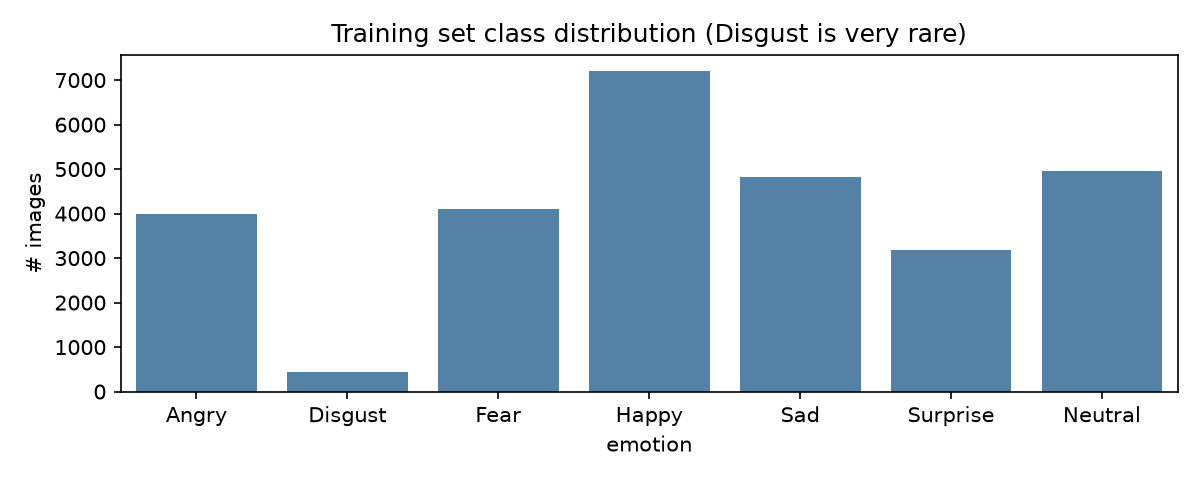
\includegraphics[width=0.85\linewidth]{../../../figures/fer_class_distribution}
\caption{FER2013 training set: class distribution.}
\label{fig:fer-dist}
\end{figure}

\begin{figure}[H]
\centering
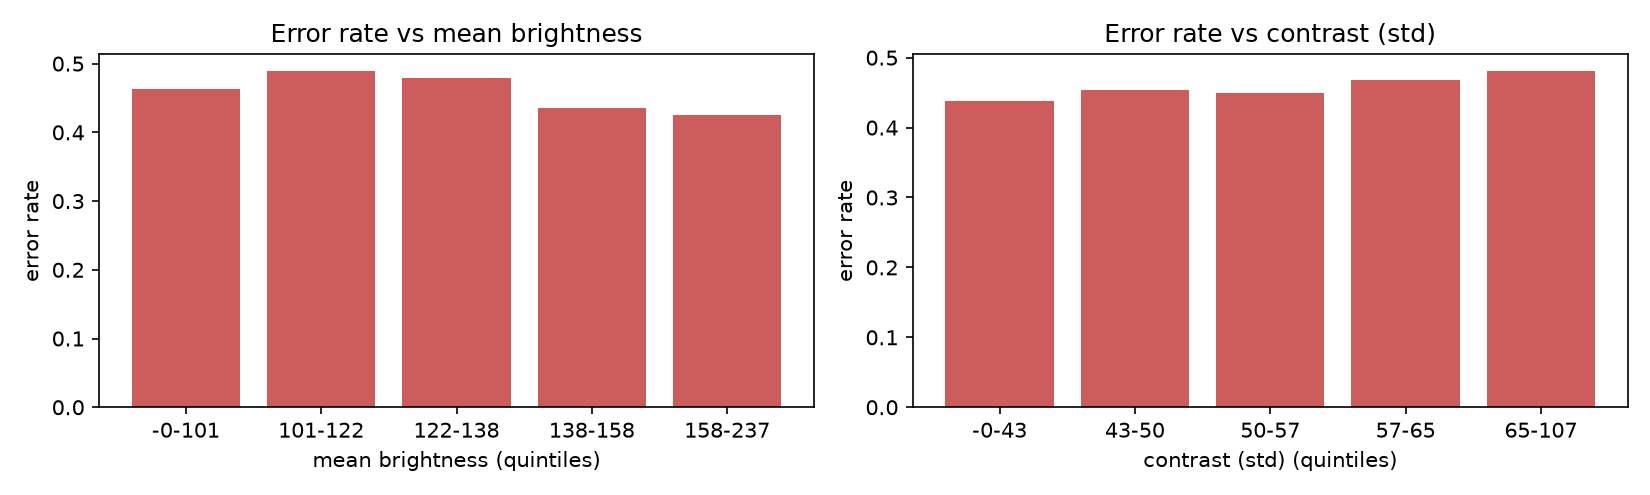
\includegraphics[width=0.85\linewidth]{../../../figures/task1_error_vs_lighting}
\caption{Error rate against lighting (HOG + SVM, validation split).}
\label{fig:err-light}
\end{figure}

Illumination and contrast have a small effect on error. We grouped validation images into quintiles of mean brightness and of contrast (pixel standard deviation) and computed the error rate of the SVM in each group. The error rate is about 0.46 to 0.49 for the three darkest quintiles and about 0.42 to 0.44 for the brightest two, and it rises slightly from about 0.44 to 0.48 as contrast increases (Figure~\ref{fig:err-light}). The effect is around five percentage points, so illumination matters but is not the main source of error.

\begin{figure}[H]
\centering
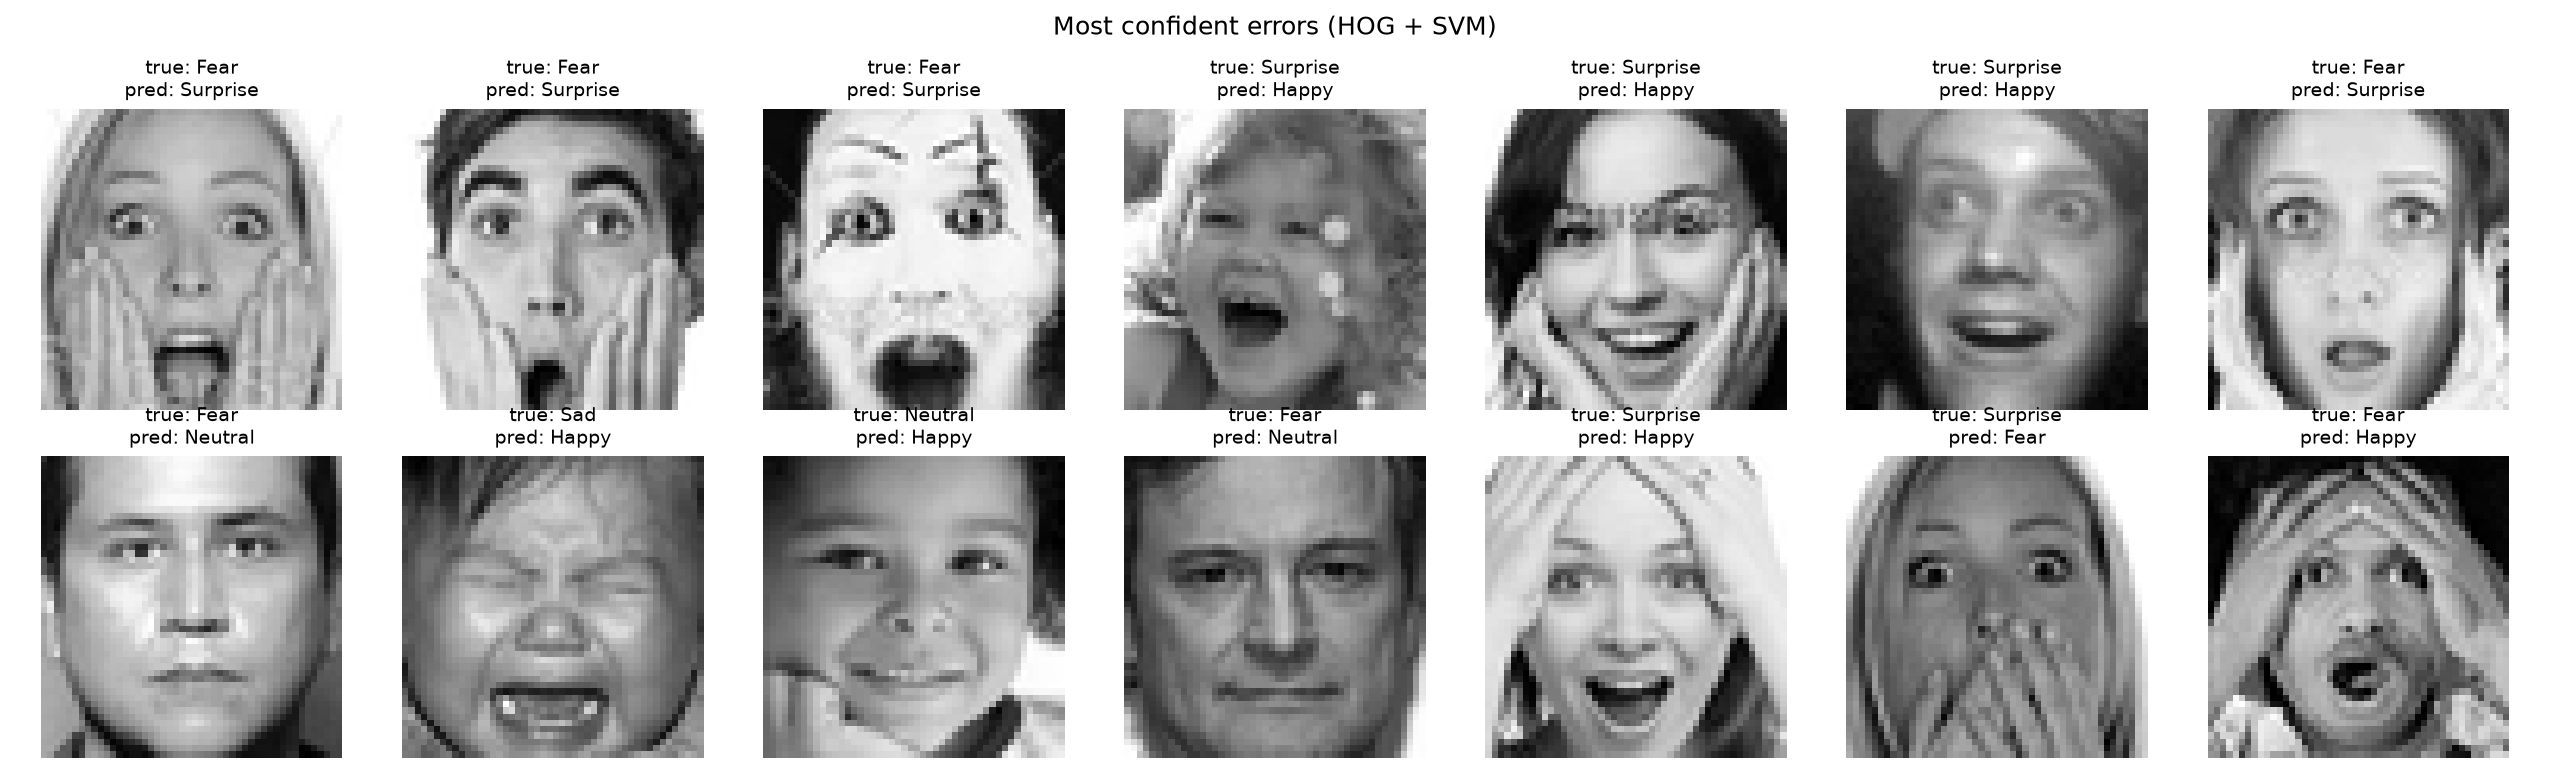
\includegraphics[width=\linewidth]{../../../figures/task1_hard_examples}
\caption{Random sample of misclassified FER2013 validation images.}
\label{fig:err-gallery}
\end{figure}

Figure~\ref{fig:err-gallery} shows recurring problems that are properties of the dataset rather than of the model: \emph{ambiguous or questionable labels} (a screaming infant labelled Angry and predicted Happy; several wide-eyed, open-mouthed faces labelled Neutral or Fear), \emph{occlusion and context} (hands over the face, hats, two faces in the crop), \emph{non-frontal pose and head tilt}, which break the aligned-face assumption of all three feature types, and \emph{population and artefacts} (infants and elderly faces, overlaid text or watermarks). The gallery is a random sample of errors, so it is qualitative evidence, not a count of mislabelled images.

\FloatBarrier
\subsection{Validation metric heatmaps (FER2013)}
\label{app:heatmaps}
\begin{figure}[H]
\centering
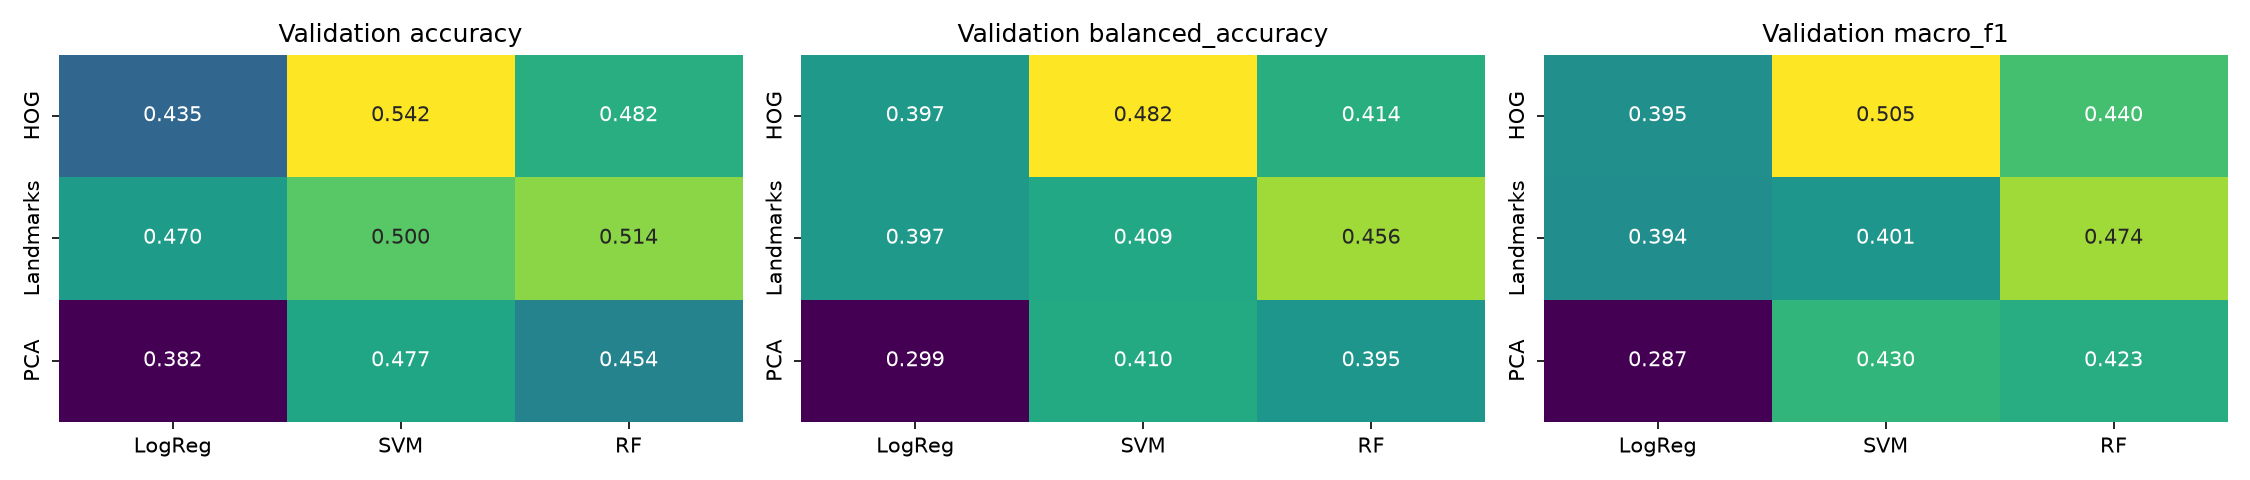
\includegraphics[width=\linewidth]{../../../figures/task1_metric_heatmaps}
\caption{Metric heatmaps of each feature--classifier combination on the FER2013 PublicTest (validation) split.}
\end{figure}

\FloatBarrier
\subsection{KDEF split and mean faces (Task 2)}
\begin{figure}[H]
  \centering
  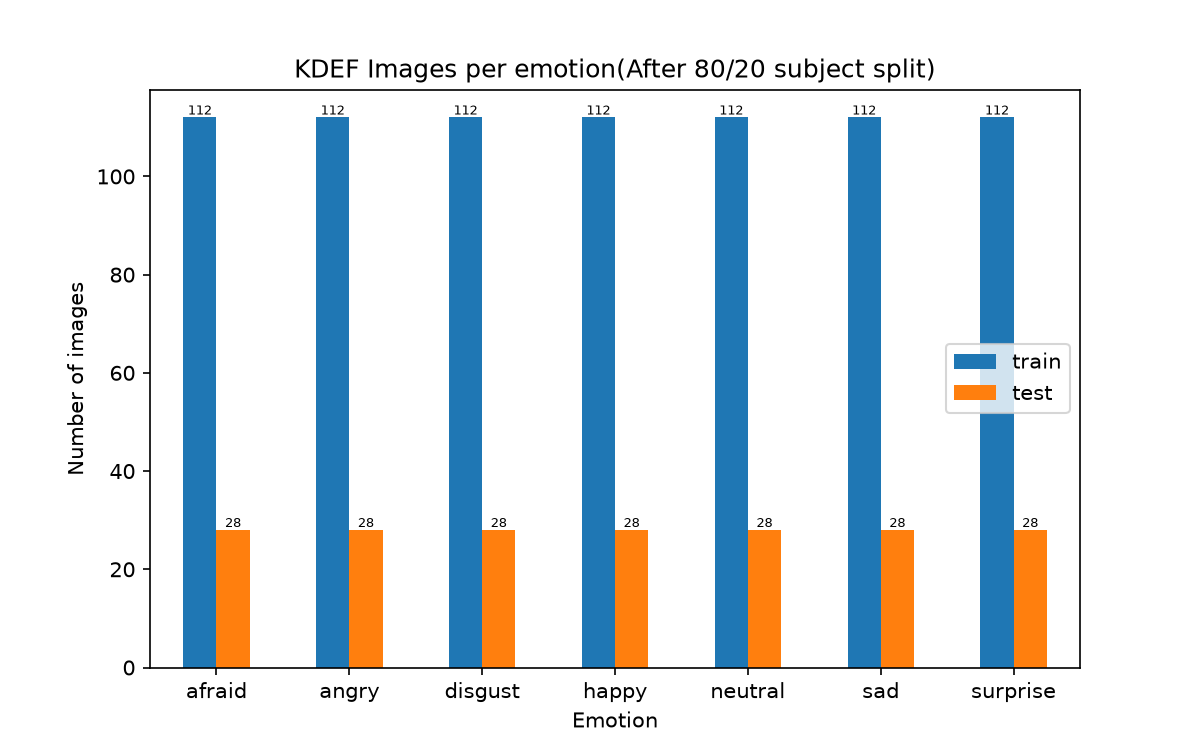
\includegraphics[width=0.5\linewidth]{../../../figures/task2_kdef_class_distribution.png}
  \caption{Number of KDEF images per emotion in the training (56 subjects) and test (14 subjects) split.}
  \label{fig:kdef-split}
\end{figure}

To understand how these alignment of these facial features could be of concern for the model, we generated the mean face for each emotion in both datasets. This was done to understand how well positioned each facial feature is in all images across the dataset. The more blurry the images are, the more inconsistent the images are in the dataset for each emotion.

\begin{figure}[H]
  \centering
  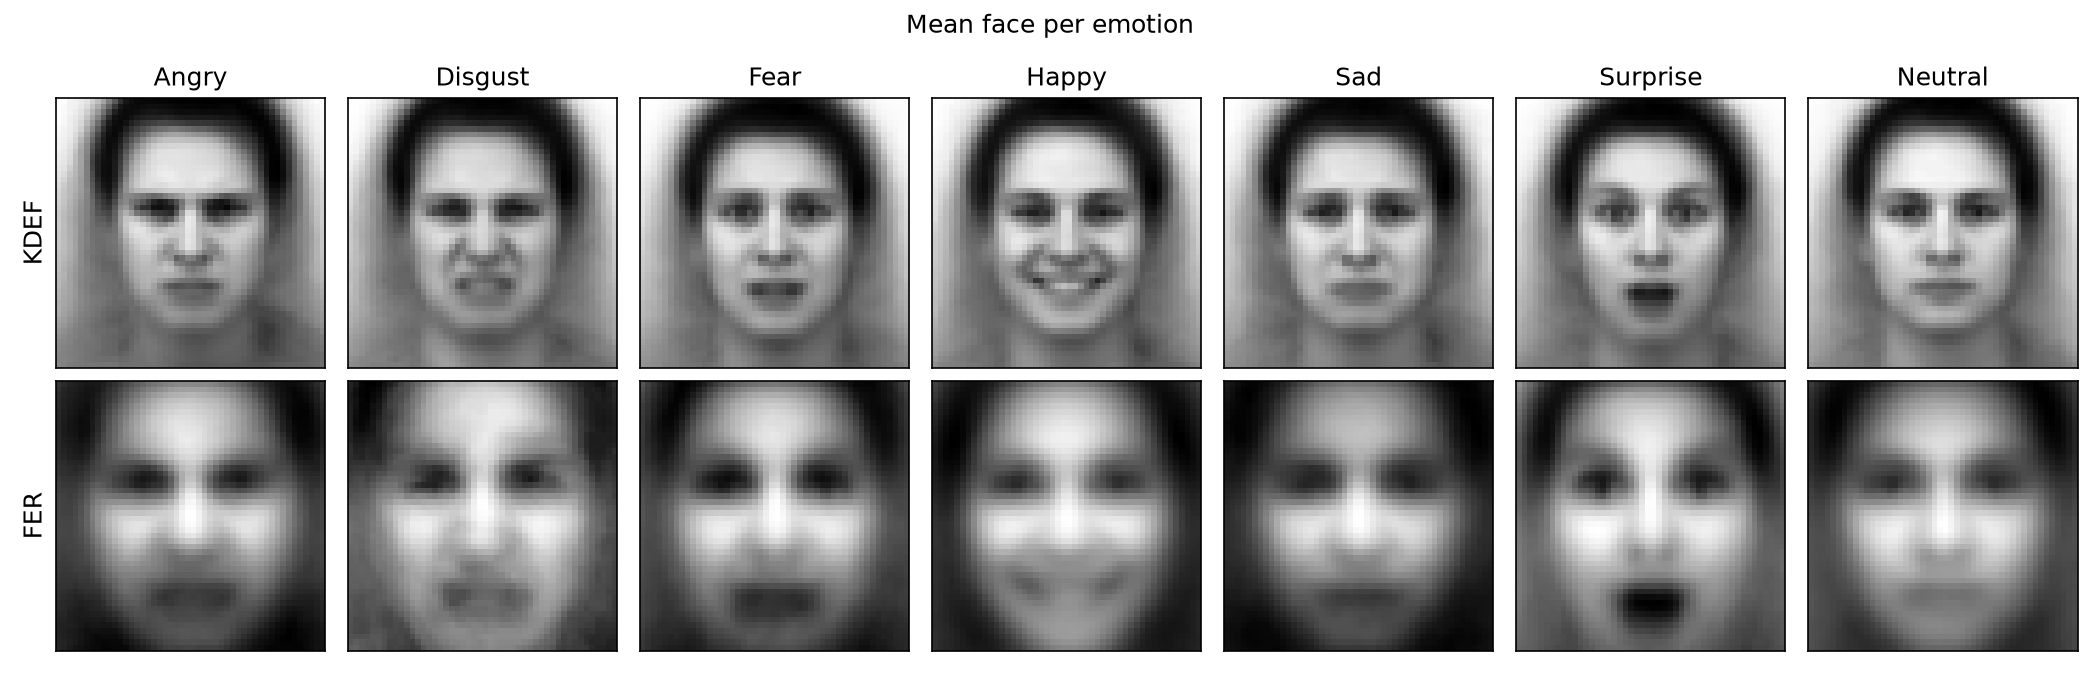
\includegraphics[width=0.72\linewidth]{../../../figures/task2_mean_faces_kdef_vs_fer.png}
  \caption{Mean face per emotion of KDEF and FER2013 training images}
  \label{fig:mean-faces}
\end{figure}

\FloatBarrier
\subsection{Domain shift and transfer examples (Task 3)}
\begin{figure}[H]
  \centering
  \begin{minipage}[t]{0.49\linewidth}
    \centering
    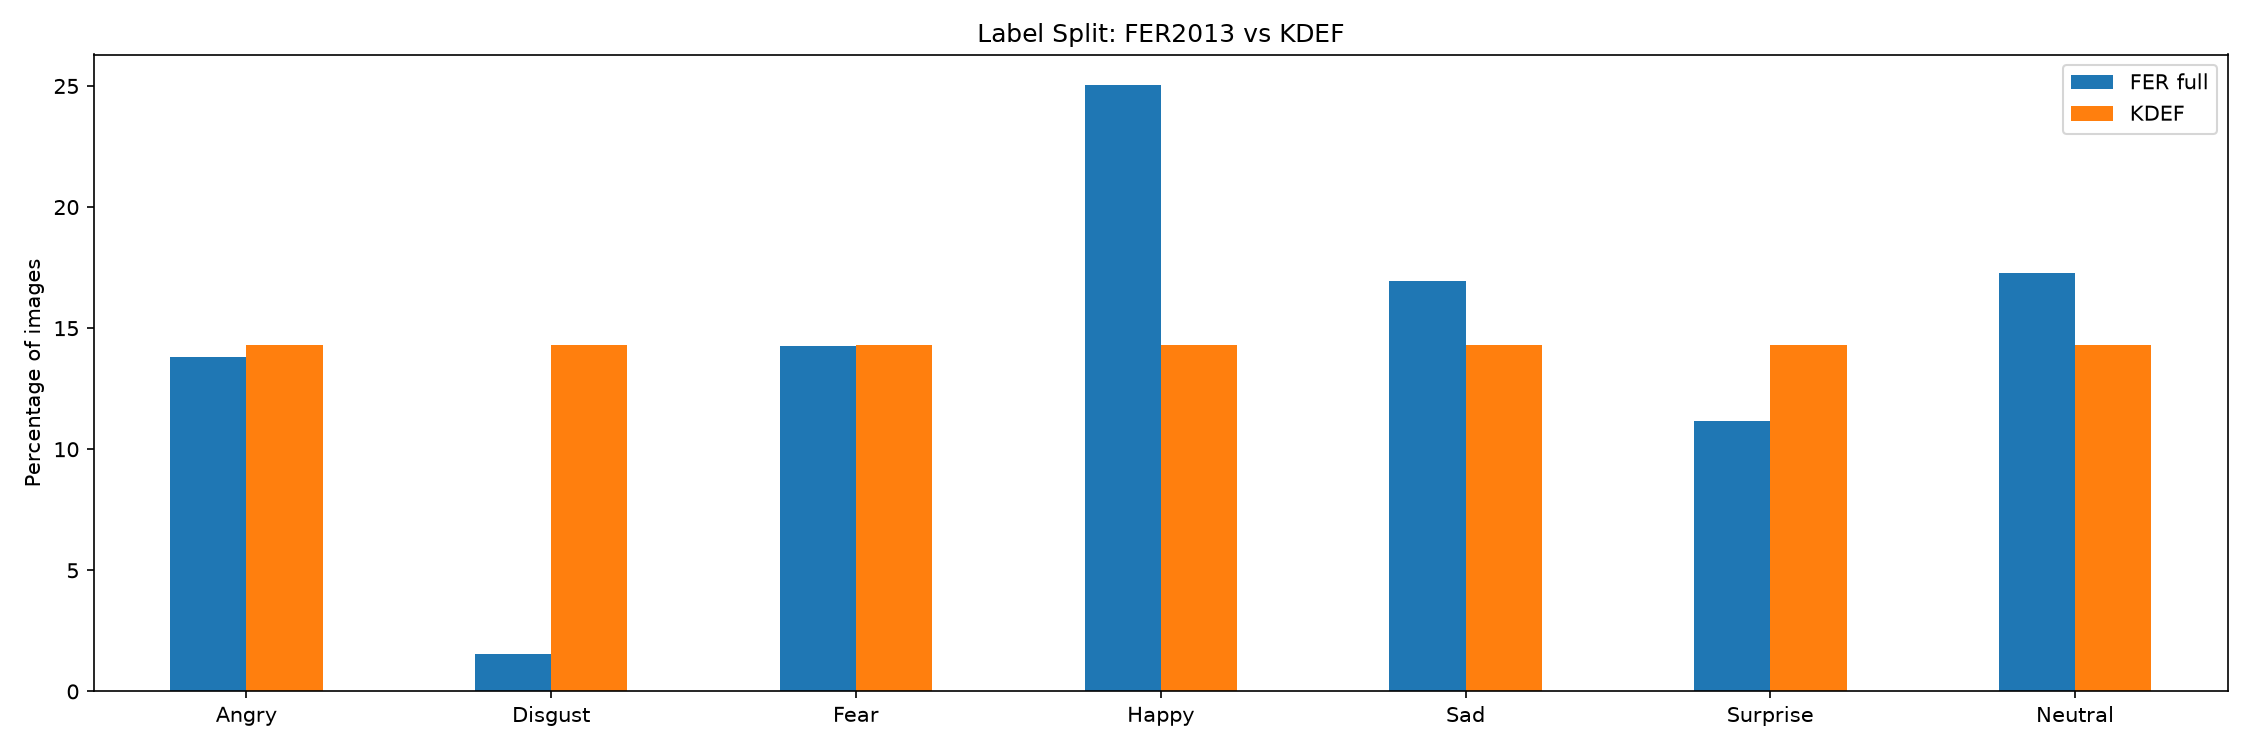
\includegraphics[width=\linewidth]{../../../figures/task3_label_split.png}
  \end{minipage}\hfill
  \begin{minipage}[t]{0.49\linewidth}
    \centering
    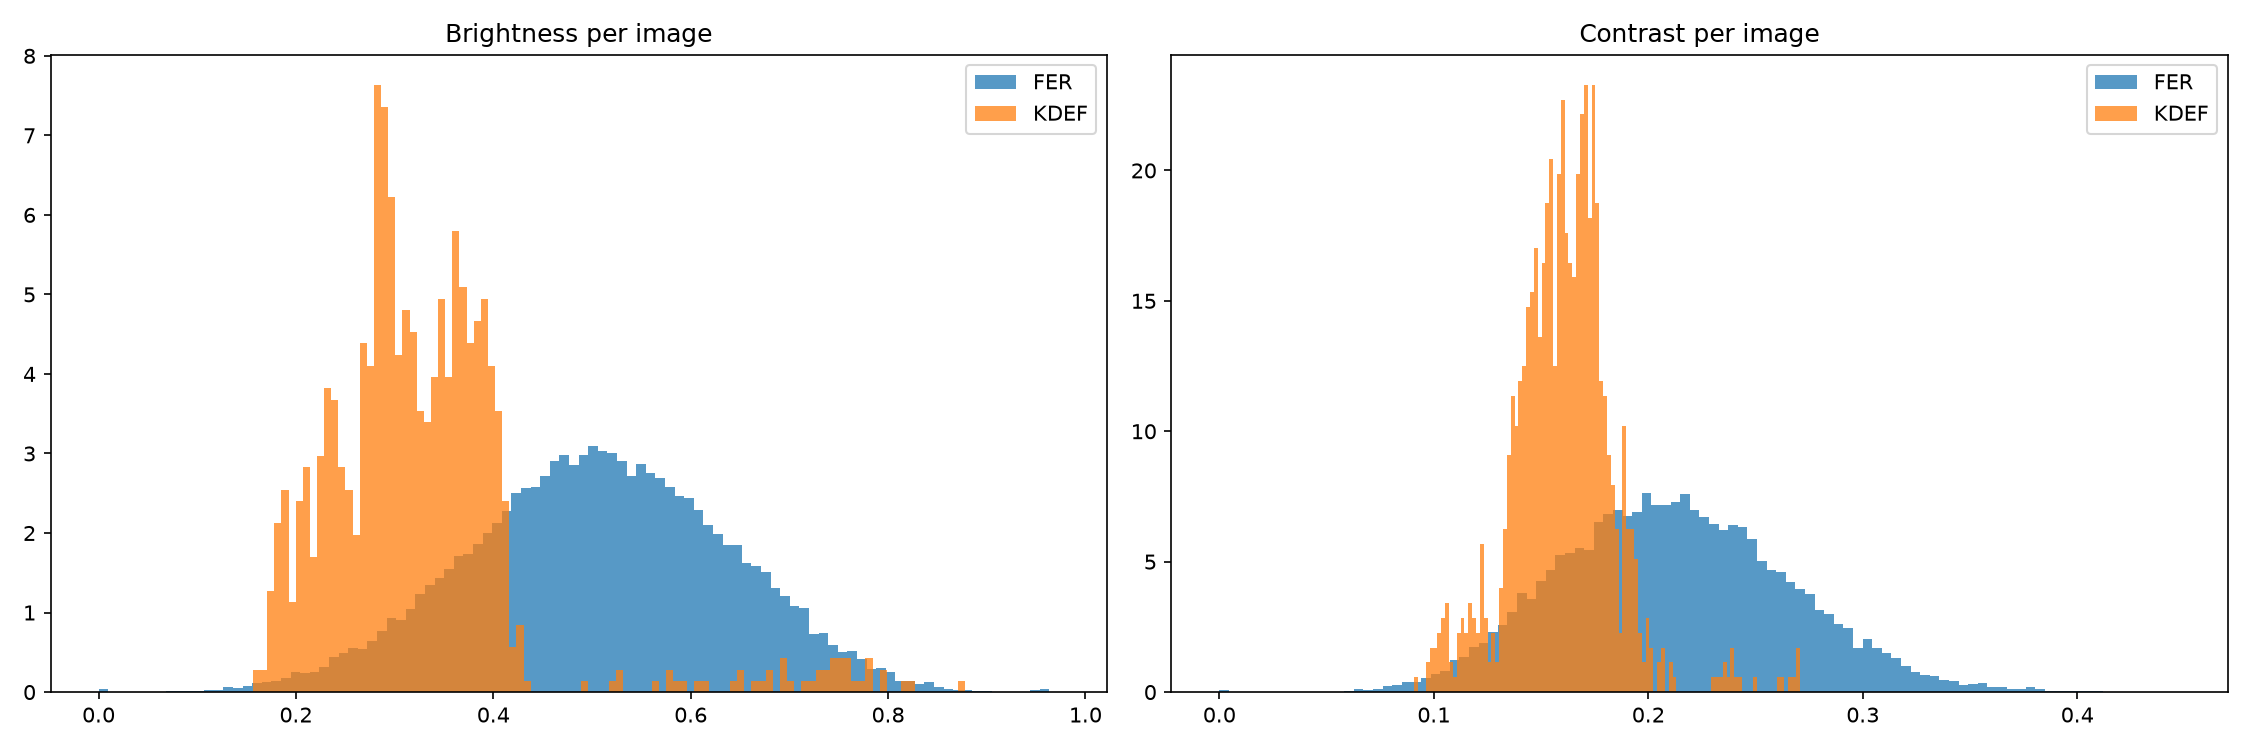
\includegraphics[width=\linewidth]{../../../figures/task3_brightness_and_contrast.png}
  \end{minipage}
  \caption{Left: share of each emotion in FER2013 and KDEF. Right: brightness and contrast of the images in both datasets.}
  \label{fig:cross-shift}
\end{figure}

\begin{figure}[H]
  \centering
  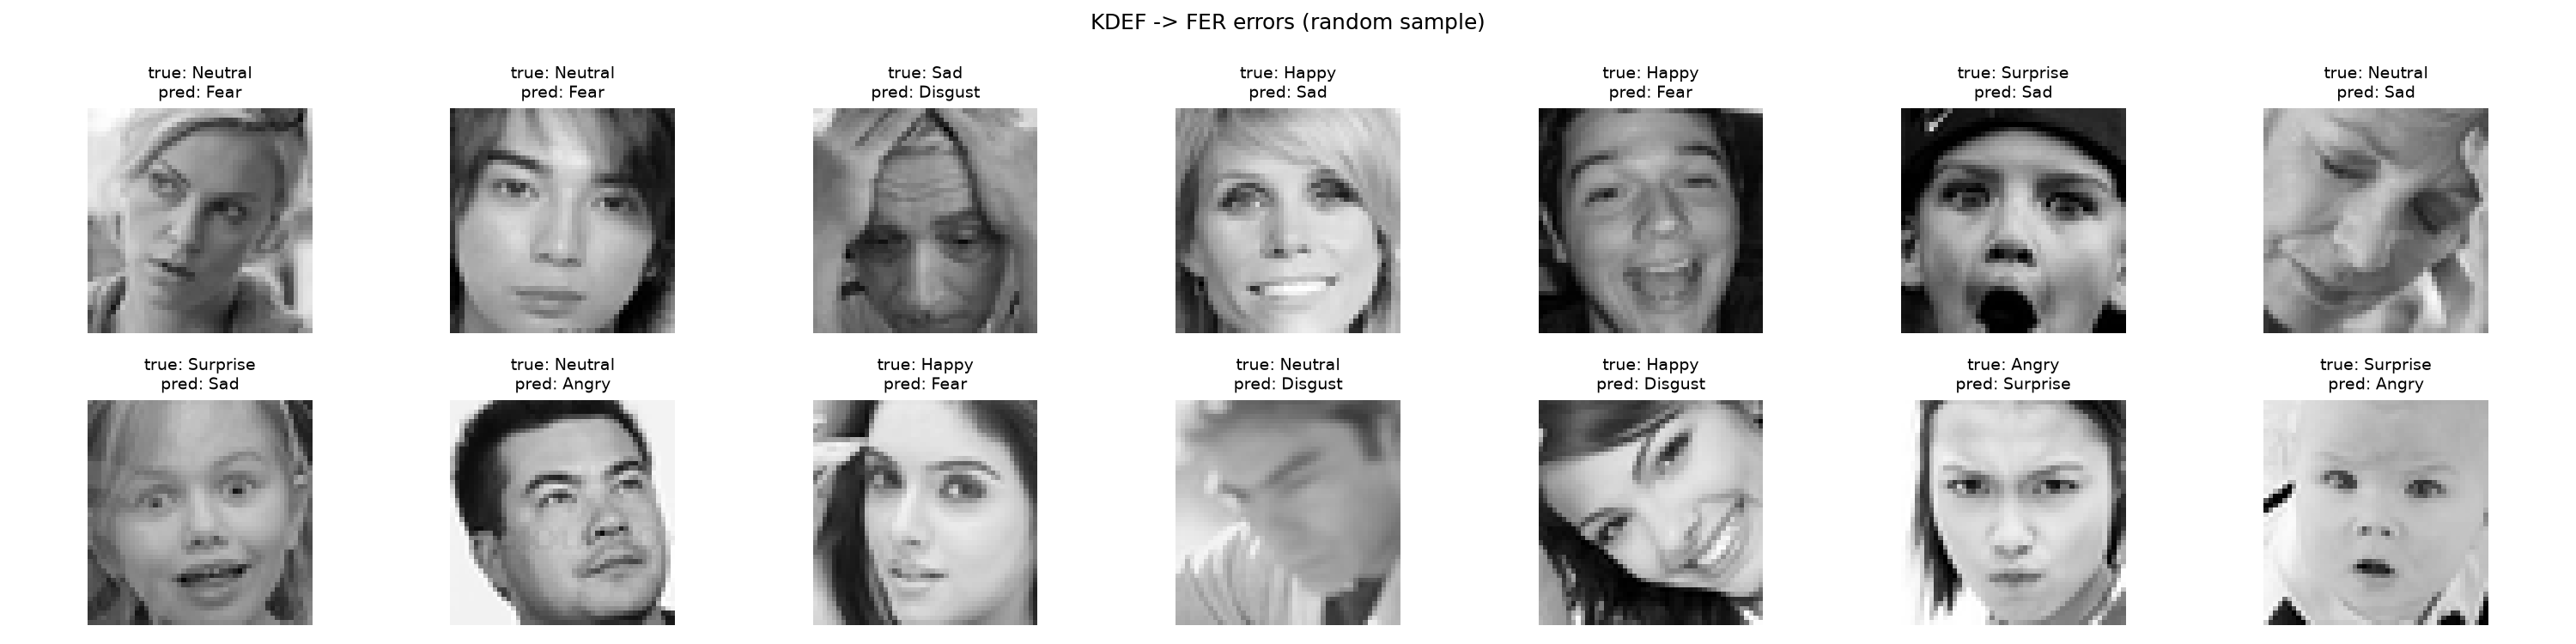
\includegraphics[width=\linewidth]{../../../figures/task3_kdef_to_fer_errors.png}
  \caption{Random FER2013 images that the KDEF-trained model gets wrong, with the true and predicted emotion.}
  \label{fig:cross-errors}
\end{figure}

\begin{figure}[H]
  \centering
  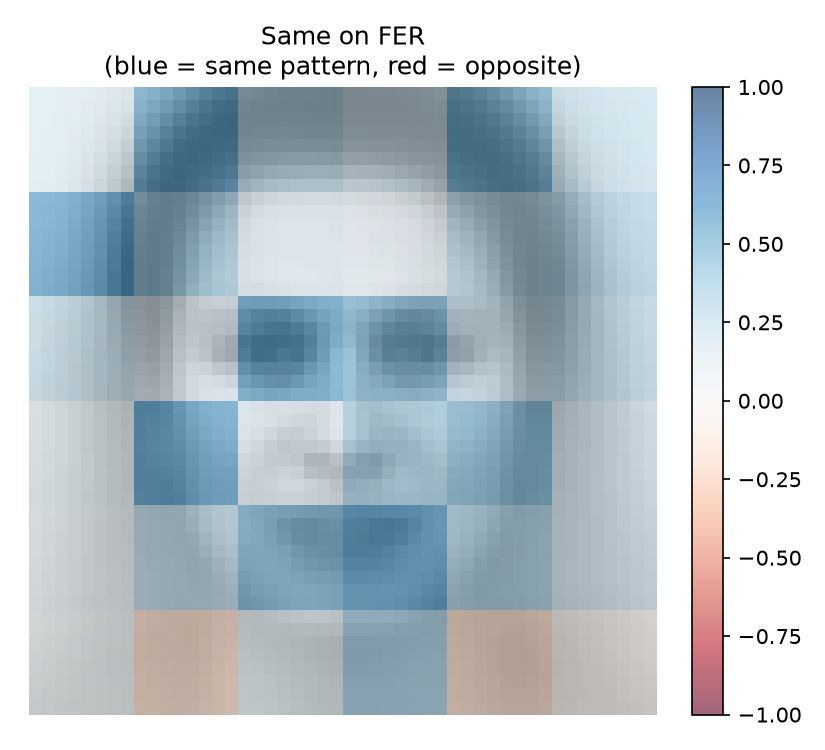
\includegraphics[width=0.38\linewidth]{../../../figures/task3_hog_feature_transfer.png}
  \caption{How well the HOG features in each region of the face transfer from KDEF to FER2013 (blue: same pattern in both datasets; red: opposite pattern).}
  \label{fig:cross-hog}
\end{figure}

\FloatBarrier
\subsection{Live demo qualitative comparison (Task 6)}
\begin{table}[H]
\centering
\scriptsize
\setlength{\tabcolsep}{5pt}
\renewcommand{\arraystretch}{1.05}

\begin{tabular}{lccc}
\toprule
Posed expression & KDEF reference & Webcam capture & Prediction \\
\midrule

Fear &
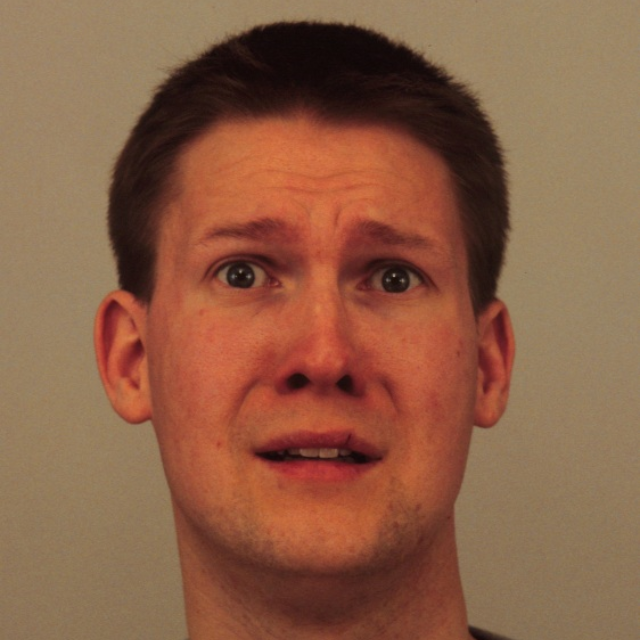
\includegraphics[height=2cm]{../../../figures/task6_empirical/kdef_fear} &
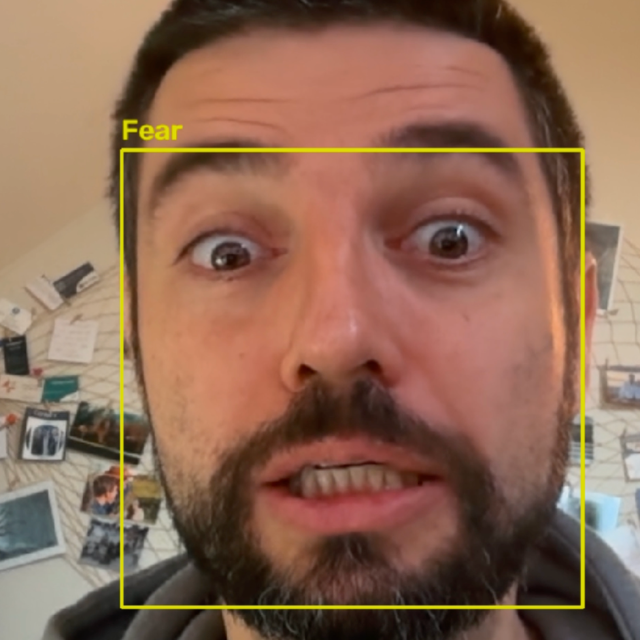
\includegraphics[height=2cm]{../../../figures/task6_empirical/webcam_fear} &
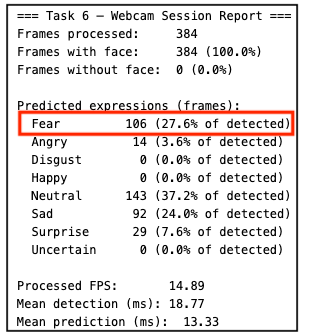
\includegraphics[height=3cm]{../../../figures/task6_empirical/results_fear} \\

Angry &
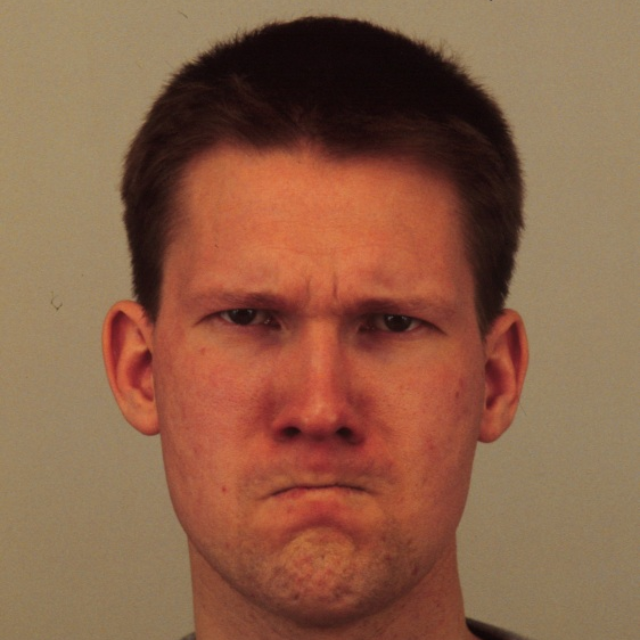
\includegraphics[height=2cm]{../../../figures/task6_empirical/kdef_angry} &
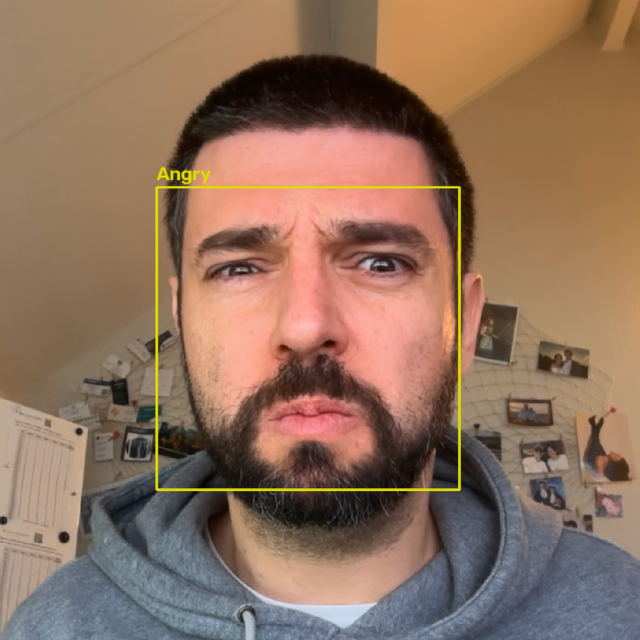
\includegraphics[height=2cm]{../../../figures/task6_empirical/webcam_angry} &
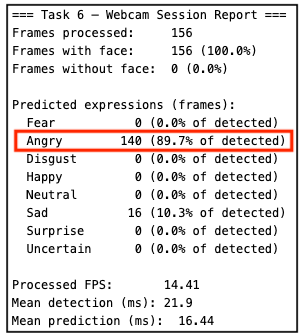
\includegraphics[height=3cm]{../../../figures/task6_empirical/results_angry}  \\

Disgust &
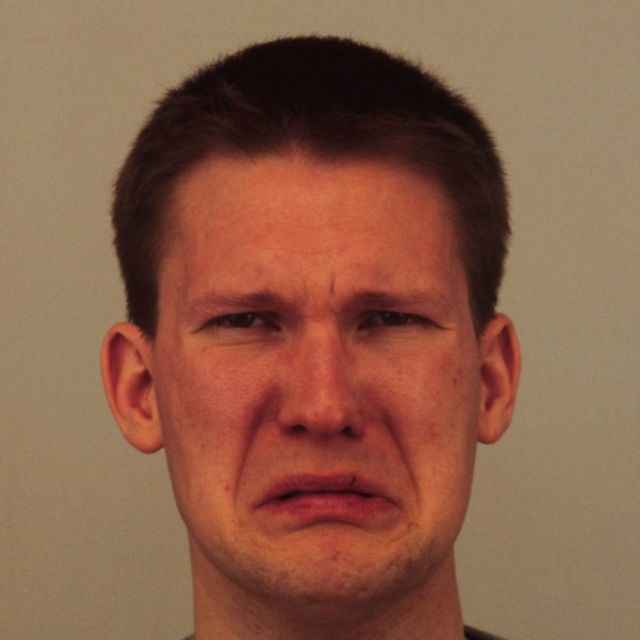
\includegraphics[height=2cm]{../../../figures/task6_empirical/kdef_disgust} &
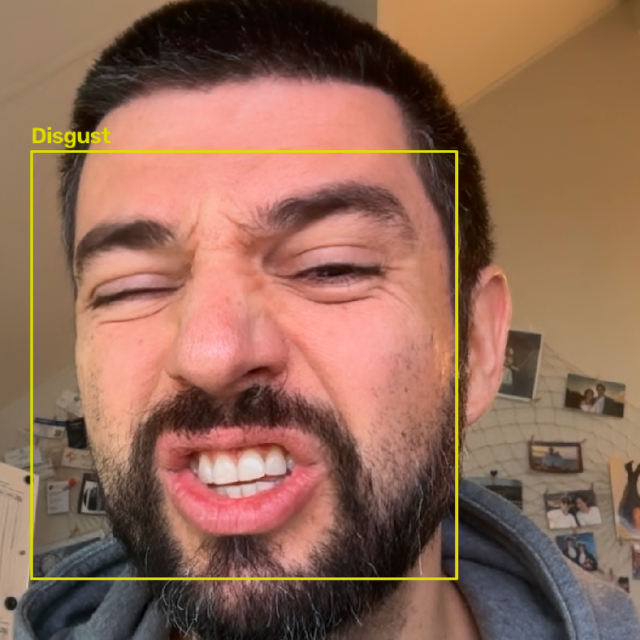
\includegraphics[height=2cm]{../../../figures/task6_empirical/webcam_disgust} &
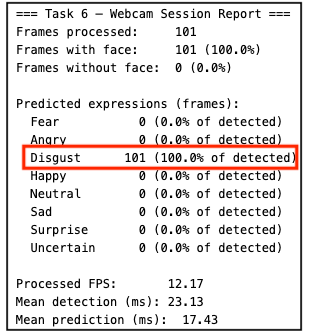
\includegraphics[height=3cm]{../../../figures/task6_empirical/results_disgust} \\

Happy &
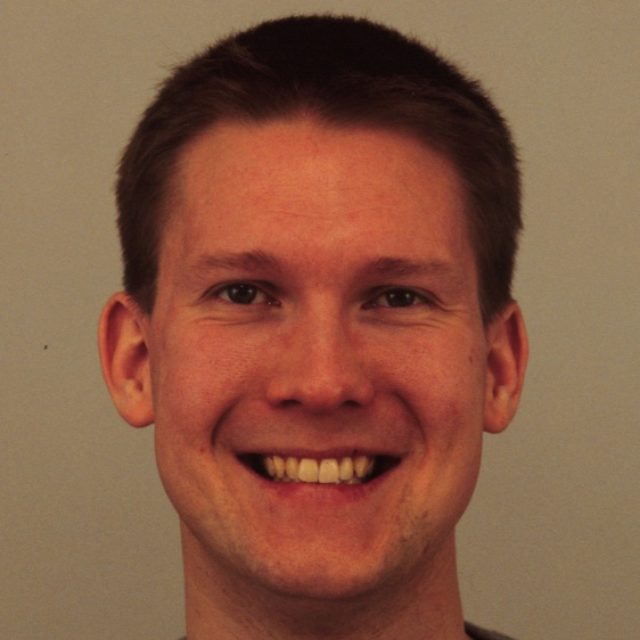
\includegraphics[height=2cm]{../../../figures/task6_empirical/kdef_happy} &
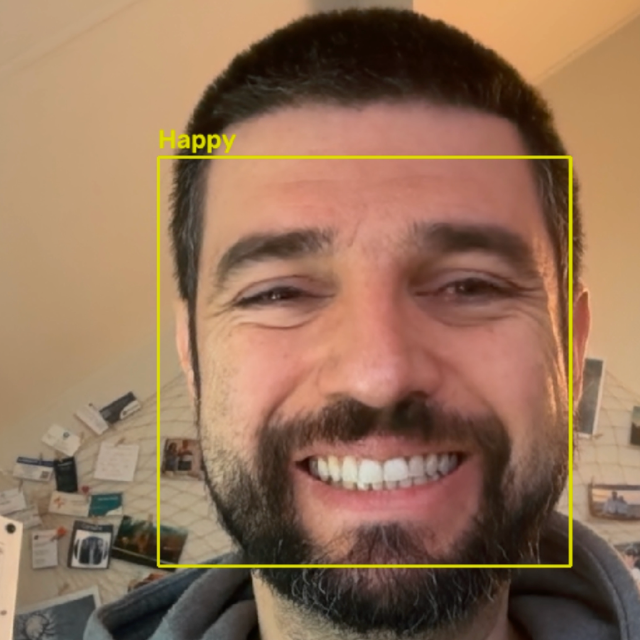
\includegraphics[height=2cm]{../../../figures/task6_empirical/webcam_happy} &
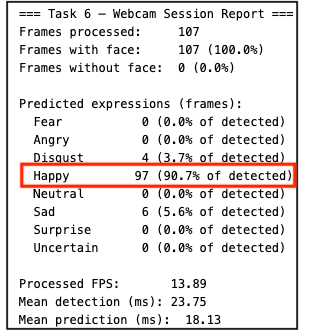
\includegraphics[height=3cm]{../../../figures/task6_empirical/results_happy} \\

Neutral &
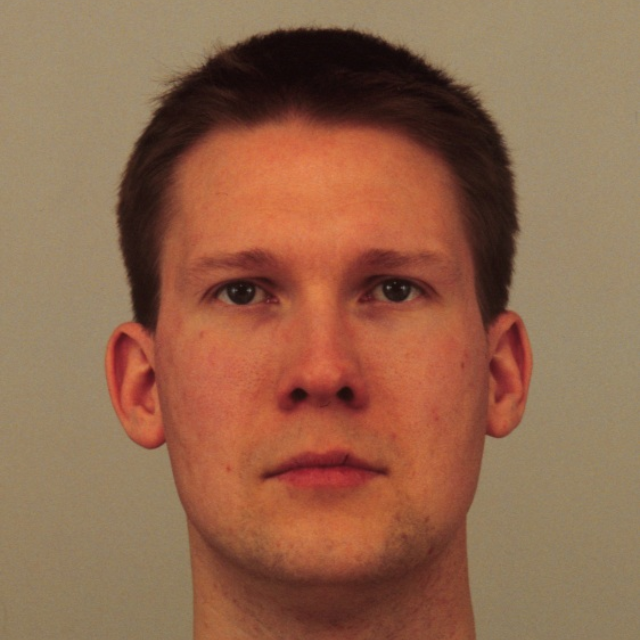
\includegraphics[height=2cm]{../../../figures/task6_empirical/kdef_neutral} &
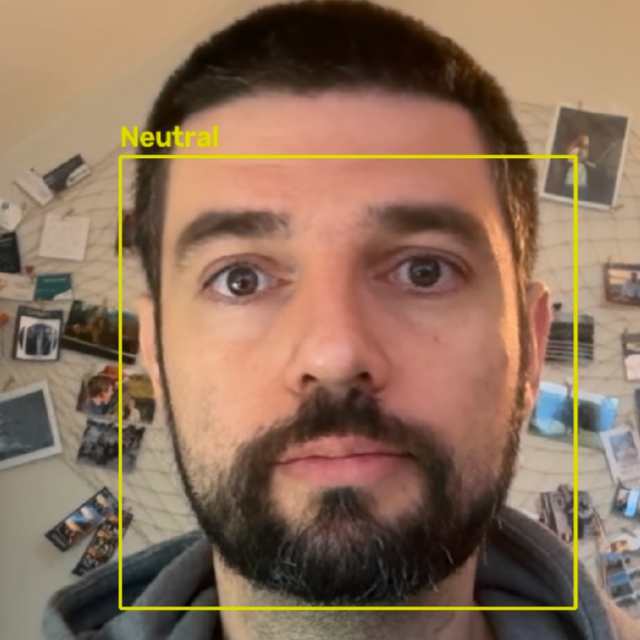
\includegraphics[height=2cm]{../../../figures/task6_empirical/webcam_neutral} &
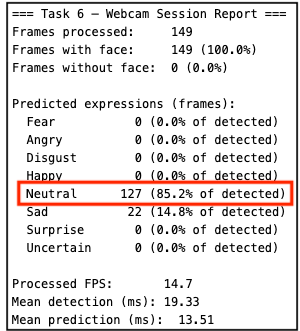
\includegraphics[height=3cm]{../../../figures/task6_empirical/results_neutral} \\

Sad &
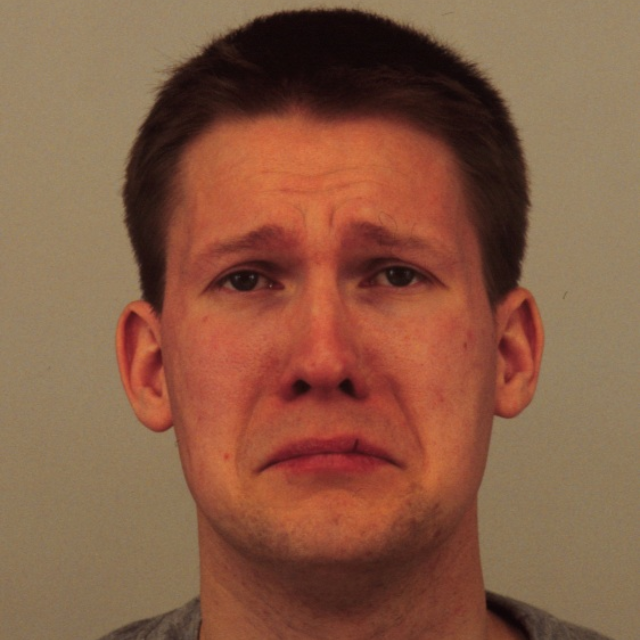
\includegraphics[height=2cm]{../../../figures/task6_empirical/kdef_sad} &
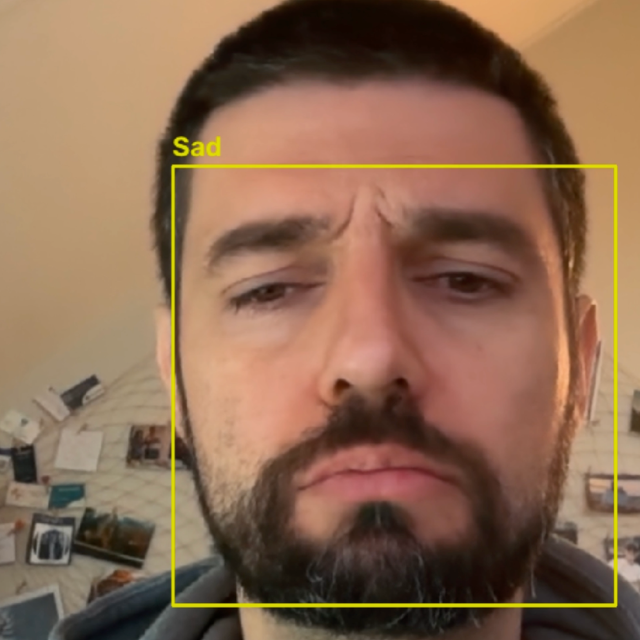
\includegraphics[height=2cm]{../../../figures/task6_empirical/webcam_sad} &
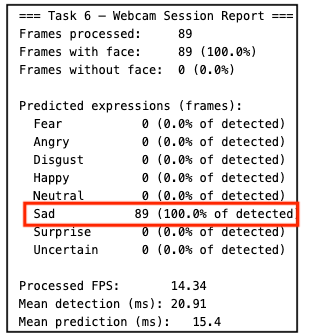
\includegraphics[height=3cm]{../../../figures/task6_empirical/results_sad} \\

Surprise &
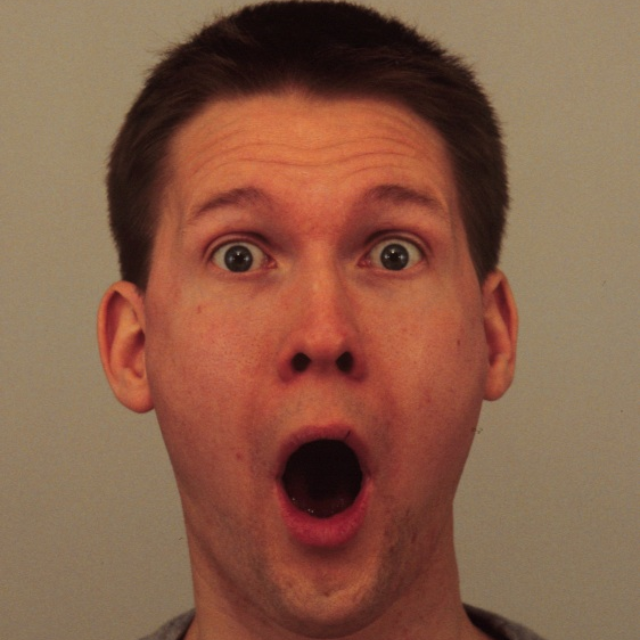
\includegraphics[height=2cm]{../../../figures/task6_empirical/kdef_surprise} &
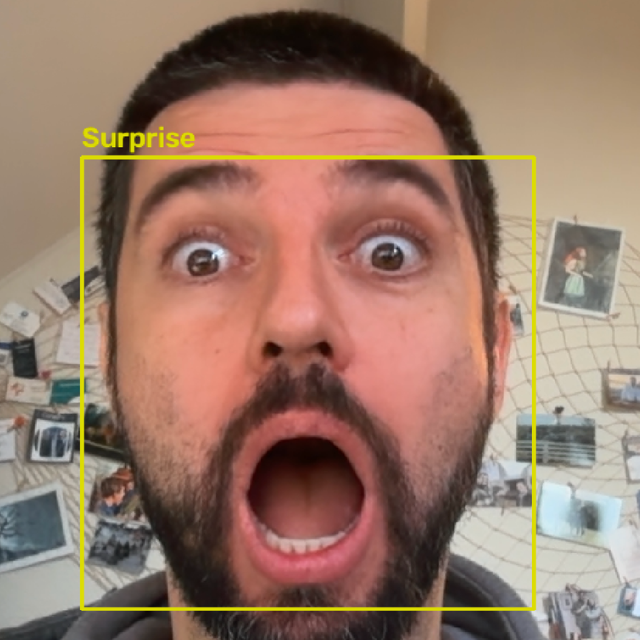
\includegraphics[height=2cm]{../../../figures/task6_empirical/webcam_surprise} &
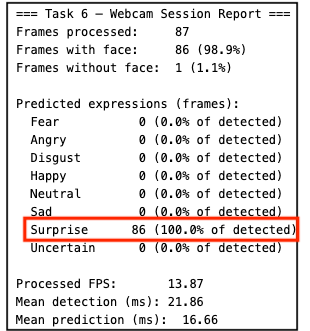
\includegraphics[height=3cm]{../../../figures/task6_empirical/results_surprise} \\

\bottomrule
\end{tabular}

\caption{
Qualitative comparison of posed KDEF expressions,
corresponding webcam expressions, and fuzzy classifier
predictions. KDEF subject M11, acquisition A, frontal pose. Webcam participant was the group member Henrique da Silva Couto.
This illustrative experiment does not establish classification accuracy.
}

\label{tab:task6_webcam_comparison}
\end{table}
